\documentclass[conference]{IEEEtran}

\usepackage{amsmath,amssymb}
\usepackage{booktabs}
\usepackage{graphicx}
\usepackage{hyperref}
\usepackage{cleveref}
\usepackage{algorithm}
\usepackage{algpseudocode}
\usepackage{xcolor}
\usepackage{enumitem}
\usepackage{caption}
\usepackage{listings}
\usepackage{microtype}
\usepackage{multirow}
\usepackage{tabularx}
\usepackage{pifont}
\usepackage{tikz}

\hypersetup{
  colorlinks=true,
  linkcolor=blue!70!black,
  citecolor=green!50!black,
  urlcolor=blue!60!black,
}

\lstset{
  language=Python,
  basicstyle=\ttfamily\scriptsize,
  keywordstyle=\color{blue!70!black}\bfseries,
  commentstyle=\color{green!50!black}\itshape,
  stringstyle=\color{red!60!black},
  breaklines=true,
  frame=single,
  framesep=2pt,
  rulecolor=\color{gray!40},
}

\crefname{lstlisting}{Listing}{Listings}
\Crefname{lstlisting}{Listing}{Listings}

\newcommand{\ncsim}{\texttt{ncsim}}
\newcommand{\dBm}{\,\text{dBm}}
\newcommand{\dB}{\,\text{dB}}
\newcommand{\mW}{\,\text{mW}}
\newcommand{\MHz}{\,\text{MHz}}
\newcommand{\GHz}{\,\text{GHz}}
\newcommand{\Mbps}{\,\text{Mbps}}
\newcommand{\MBps}{\,\text{MB/s}}
\newcommand{\cmark}{\ding{51}}
\newcommand{\xmark}{\ding{55}}

\title{\ncsim{}: A Lightweight Simulator for Networked\\Edge Computing with Wireless Interference Modeling}
\author{
\IEEEauthorblockN{Anonymous Author(s)}
\IEEEauthorblockA{Affiliation withheld for double-blind review}
}

\begin{document}
\maketitle

%% ============================================================
\begin{abstract}
Evaluating DAG task schedulers for wireless edge computing requires
jointly modeling compute placement and wireless interference, yet
existing tools treat them in isolation.  This gap leads to
\emph{rank inversions}: the scheduler that appears optimal under an
interference-free model can be the worst choice under realistic
wireless conditions.  We present \ncsim{}, a lightweight
discrete-event simulator that bridges this gap by combining DAG
workflow scheduling with physically-grounded IEEE~802.11 CSMA/CA
interference modeling in a single Python package.  A 108-run
factorial experiment reveals rank inversions in 27.8\% of scenarios,
with the interference-free-optimal scheduler producing up to
$2.7\times$ worse makespan than a simple round-robin baseline;
scaling to a 100-node random geometric graph raises the inversion
rate to 50\%.  These rank inversions show that
interference-free evaluation can select the wrong algorithm
entirely, justifying the design and use of \ncsim{}.
\end{abstract}

%% ============================================================
\section{Introduction}
\label{sec:intro}

Edge and fog computing architectures distribute computation across
heterogeneous nodes connected by networks of varying capacity and
reliability~\cite{shi2016edge}.  Effective task scheduling in these
environments requires co-optimizing compute placement and network transport:
a task placement that minimizes computation time may incur excessive data
transfer costs, while a network-aware placement may underutilize fast
processors.

Existing simulation tools address parts of this problem.  Network simulators
such as ns-3~\cite{ns3} and OMNeT++~\cite{omnetpp} provide detailed protocol
stacks but are heavyweight, complex to configure, and lack native support for
DAG-based task scheduling.  Conversely, task scheduling simulators such as
SimGrid~\cite{simgrid}, WRENCH~\cite{wrench}, and CloudSim~\cite{cloudsim}
model workflows and compute resources but typically abstract the network as
point-to-point links with fixed bandwidths, omitting wireless contention,
interference, and multi-hop effects.  Edge-specific tools like
iFogSim~\cite{ifogsim} and EdgeCloudSim~\cite{edgecloudsim} add
domain-specific features but use simplified wireless models that do not
capture the distance-dependent rates, CSMA contention, or hidden terminal
interference that characterize real 802.11 deployments.

We present \ncsim{},\footnote{Repository URL withheld for double-blind review; the artifact will be released publicly upon acceptance.}
an open-source, lightweight, flow-level discrete-event simulator that
combines DAG workflow scheduling with physically-grounded 802.11 WiFi
models in a single Python package.  \ncsim{} deliberately occupies the
space between packet-level network simulators (ns-3, OMNeT++) and
workflow simulators (SimGrid, WRENCH, CloudSim, iFogSim): more
wireless-realistic than workflow tools, but much lighter than ns-3 for
scheduler sweeps.

To demonstrate why this niche matters, we use \ncsim{} to run a 108-run
factorial study and find that the scheduler appearing optimal under an
interference-free model is outperformed under realistic CSMA/CA
conditions in 27.8\% of scenarios, a \emph{rank inversion}.  In the
most striking case, the HEFT scheduler produces $2.7\times$ worse
makespan than a simple round-robin baseline, yet an interference-free
evaluation would confidently select HEFT.  This result is infeasible
to produce with either class of existing tool, and it establishes
that realistic wireless modeling is essential for evaluating edge
computing schedulers.

The contributions are:

\begin{enumerate}[itemsep=2pt,leftmargin=*]
\item \textbf{\ncsim{} simulator:} a modular architecture combining DAG
  scheduling (HEFT, CPOP, round-robin) with 802.11 WiFi models
  (log-distance path loss, MCS rate adaptation, Bianchi CSMA/CA
  contention, hidden terminal SINR degradation, multi-hop routing with
  dynamic bandwidth sharing) in ${\sim}5{,}500$ lines of Python.
\item \textbf{Three-stage validation ladder:} nine internal experiments
  matching analytical predictions exactly, reproduction of Bianchi's
  published results~\cite{bianchi2000}, and cross-validation against
  ns-3 packet-level simulations (mean error 4\%).
\item \textbf{Rank inversion finding:} a 108-run factorial on grid networks
  revealing that interference-free evaluation produces wrong scheduler
  rankings in 27.8\% of scenarios.
\item \textbf{Scalability confirmation:} a 36-run study on a 100-node
  random geometric graph with 30--50 task DAGs, where the rank inversion
  rate rises to 50\%.
\end{enumerate}

\Cref{sec:related,sec:arch,sec:model,sec:engine} survey related work and
describe \ncsim{}'s architecture, system model, and simulation engine.
\Cref{sec:validation} validates the WiFi model, and \Cref{sec:eval}
presents the experimental evaluation.  \Cref{sec:conclusion} discusses
implications and future directions.


%% ============================================================
\section{Related Work}
\label{sec:related}

We situate \ncsim{} at the intersection of DAG scheduling research and
wireless network simulation.  The key gap is not any single prior system
but the combination our target users need: DAG-aware scheduling, wireless
CSMA/CA and hidden-terminal modeling, and lightweight sweepability in one
tool.  \Cref{tab:sim_comparison} summarizes the comparison.

\textbf{DAG scheduling and workflow systems.}
DAG scheduling has a rich history in parallel computing, from
list-scheduling and dynamic-level scheduling to HEFT and
CPOP~\cite{Adam1974ListSchedules,KwokAhmad1999Survey,Sih1993DLS,heft}.
Benchmarking and parametric scheduler design tools such as SAGA, PISA,
and parametric decomposition enable adversarial search and systematic
ablation~\cite{Coleman2024PISA,SAGARepo,Coleman2024Parametric}.
Dispersed and edge execution systems (Jupiter, Tactical Jupiter, and
throughput-oriented extensions) integrate DAG scheduling with
profiling and orchestration on real
clusters~\cite{Ghosh2021Jupiter,Poylisher2021TacticalJupiter,Zhao2021TPHEFT}.
None of these model wireless contention at the physical layer.

\textbf{Network simulators and wireless/edge DAG systems.}
ns-3~\cite{ns3} and OMNeT++~\cite{omnetpp} provide detailed WiFi, LTE,
and TCP/IP stacks with high-fidelity channel models, but they are
heavyweight: configuring custom DAG scheduling requires external workflow
engines and C++ glue code, and packet-level simulation times make large
parameter sweeps prohibitive.  A growing body of edge/IoT DAG scheduling
work tackles heterogeneous devices and MEC
offloading~\cite{Suryavansh2020IBOT,Li2022IBDASH,Li2024MTEC,Yi2017LAVEA,Zhang2019HeteroEdge,Lin2019Petrel,Liang2021JointOffloading,Li2024EnergyConstrained,Long2025SecDS,Chiang2016FogIoT,Chiang2017Fog10Q,Kim2020CodedEdge},
but it typically assumes abstract link rates rather than modeling the
CSMA/CA and hidden-terminal phenomena that dominate real 802.11 channels.

\textbf{Workflow and edge simulators.}
SimGrid~\cite{simgrid}, WRENCH~\cite{wrench}, and CloudSim~\cite{cloudsim}
support DAG workflows natively but model networks as links with fixed or
analytically-derived bandwidths.  This abstraction fits wired data
centers but omits wireless contention, hidden terminals, and spatial
reuse.  Edge-specific tools such as iFogSim~\cite{ifogsim} and
EdgeCloudSim~\cite{edgecloudsim} add latency-sensitive placement and
mobility but retain simplified wireless models.  \ncsim{} fills the
resulting gap by combining DAG-aware scheduling with physically-grounded
802.11 wireless models in a lightweight Python package, providing a
controlled environment where wireless effects can be systematically
varied and their impact on scheduling quality precisely measured.

\begin{table}[t]
\centering
\caption{Simulator comparison. \ncsim{} uniquely combines DAG-native
scheduling with CSMA/CA and hidden terminal modeling at flow-level
granularity.}
\label{tab:sim_comparison}
\setlength{\tabcolsep}{3.5pt}
\begin{tabular}{@{}lcccccc@{}}
\toprule
\textbf{Tool} & \rotatebox{70}{\textbf{DAG}} &
  \rotatebox{70}{\textbf{WiFi}} &
  \rotatebox{70}{\textbf{CSMA}} &
  \rotatebox{70}{\textbf{Hid.\ Term.}} &
  \rotatebox{70}{\textbf{Pkt-Level}} &
  \rotatebox{70}{\textbf{Sweep}} \\
\midrule
ns-3~\cite{ns3}          & \xmark & \cmark & \cmark & \cmark & \cmark & High \\
OMNeT++~\cite{omnetpp}   & \xmark & \cmark & \cmark & \cmark & \cmark & High \\
SimGrid~\cite{simgrid}   & \cmark & \xmark & \xmark & \xmark & \xmark & Low \\
WRENCH~\cite{wrench}     & \cmark & \xmark & \xmark & \xmark & \xmark & Low \\
CloudSim~\cite{cloudsim} & \cmark & \xmark & \xmark & \xmark & \xmark & Low \\
iFogSim~\cite{ifogsim}   & \cmark & \xmark & \xmark & \xmark & \xmark & Med \\
EdgeCloudSim~\cite{edgecloudsim} & \xmark & \cmark & \xmark & \xmark & \xmark & Med \\
\textbf{\ncsim{}}        & \cmark & \cmark & \cmark & \cmark & \xmark & \textbf{Low} \\
\bottomrule
\end{tabular}
\end{table}

%% ============================================================
\section{Architecture}
\label{sec:arch}

In this section, we describe the architecture of \ncsim{}, which is organized
around a layered discrete-event simulation (DES) engine with pluggable
components for scheduling, routing, and interference modeling.
\Cref{fig:architecture} illustrates the data flow from scenario
specification through simulation to output traces.

\begin{figure}[t]
\centering
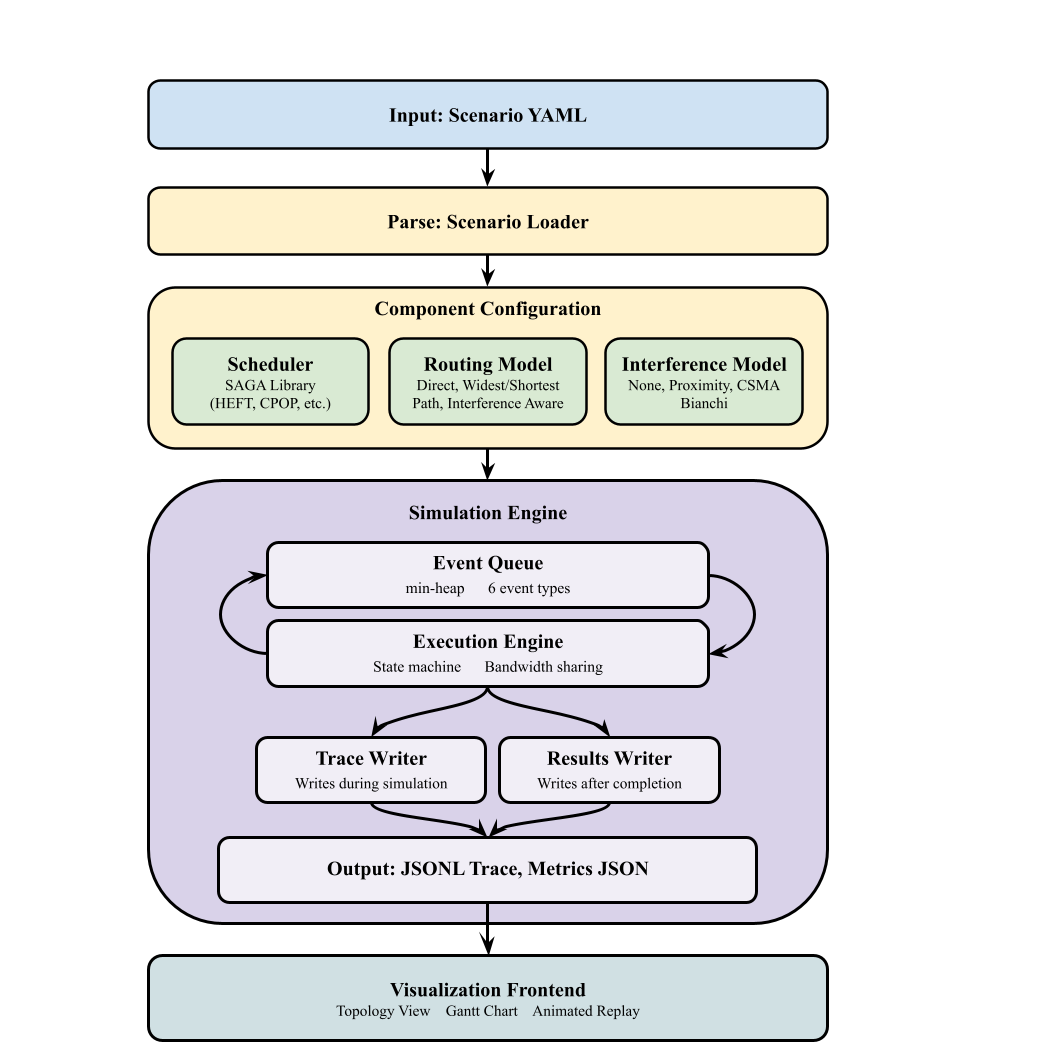
\includegraphics[width=\columnwidth]{figures/architecture.png}
\caption{High-level architecture of \ncsim{}.}
\label{fig:architecture}
\end{figure}

\subsection{Design Goals}

Four principles guide \ncsim{}.
\textbf{Determinism:} rounding all simulation times to microsecond precision ($10^{-6}$\,s) yields bit-identical results across runs and platforms.
\textbf{Modularity:} six abstract base classes (\Cref{tab:abstractions}) decouple schedulers, routing, and interference models so swapping one does not touch the others.
\textbf{Simplicity:} scenarios are declarative YAML; the whole simulator is ${\sim}5{,}500$ lines of Python with minimal dependencies.
\textbf{Physical grounding:} link bandwidths are derived from RF parameters (transmit power, frequency, path loss exponent), so link rates are physically consistent with node positions rather than specified as arbitrary constants.

\subsection{Scope and Assumptions}

\ncsim{} targets macroscopic scheduling decisions rather than protocol
engineering.  It intentionally omits packet-level simulation, physical-layer
channel dynamics (fading, OFDM), mobility, and multi-slot compute
parallelism, retaining the phenomena that most affect scheduling: CSMA/CA
contention, hidden terminals, and MCS rate adaptation.
\Cref{tab:scope} summarizes the modeling scope.

\begin{table}[t]
\centering
\caption{Scope of validity: phenomena modeled by \ncsim{} and their
impact on scheduling studies.}
\label{tab:scope}
\begin{tabular}{@{}lll@{}}
\toprule
\textbf{Phenomenon} & \textbf{Status} & \textbf{Impact} \\
\midrule
CSMA/CA contention    & Modeled (Bianchi)       & High \\
Hidden terminals      & Modeled (SINR)          & High \\
MCS rate adaptation   & Modeled (11n/ac/ax)     & Medium \\
Path loss             & Modeled (log-distance)  & High \\
Pkt-level dynamics    & Not modeled             & Low$^\dagger$ \\
TCP slow-start        & Not modeled             & Medium$^\ddagger$ \\
Fading / mobility     & Optional (log-normal)   & Low$^\S$ \\
Multi-slot parallelism & Not modeled            & App-dependent \\
\bottomrule
\multicolumn{3}{@{}l}{\scriptsize $^\dagger$For bulk transfers.
  $^\ddagger$For short flows. $^\S$For static deployments.}
\end{tabular}
\end{table}

\ncsim{}'s flow-level abstraction targets the regime of scheduler
evaluation with bulk DAG edges (10\,MB-class payloads), where
steady-state throughput dominates and TCP slow-start is negligible.  The
Bianchi saturation model and capture-threshold hidden-terminal model are
the right level of fidelity for that regime: they capture the
first-order effects that change scheduling outcomes (channel time-share
and SINR-driven rate drops) without the cost of packet-level simulation.
We use deterministic path loss throughout to isolate contention and
hidden-terminal effects from fading and mobility; stochastic channels
are available but are not the focus of this paper.

\subsection{Key Abstractions}

Six abstract base classes (\Cref{tab:abstractions}) let researchers plug
in their own schedulers, routing models, or interference models without
touching the core event engine; every component used in
\Cref{sec:eval} is itself an instance of these interfaces.

\begin{table}[t]
\centering
\caption{Pluggable abstractions in \ncsim{}.}
\label{tab:abstractions}
\begin{tabular}{@{}lp{4.8cm}@{}}
\toprule
\textbf{ABC} & \textbf{Implementations} \\
\midrule
Scheduler & Manual, RoundRobin, HEFT, CPOP \\
RoutingModel & Direct, WidestPath, ShortestPath \\
InterferenceModel & None, CSMA Bianchi \\
LinkModel & Static \\
QueueModel & FIFO \\
DAGSource & Single, Multi \\
\bottomrule
\end{tabular}
\end{table}

\subsection{Visualization and Tooling}
\label{sec:viz}

\ncsim{} includes a React/D3 web-based visualization frontend with three
views: a \textbf{network topology view} showing nodes, links, and active
transfers; a \textbf{Gantt chart} of task execution and transfer timelines
per node; and an \textbf{animated replay} with playback controls for
observing bandwidth recalculation cascades.  Simulation output is written
in JSONL trace format (one JSON object per event) for integration with
external analysis tools.  The command-line interface supports batch
execution, facilitating the automated parameter sweeps used throughout
\Cref{sec:eval}.

\subsection{Artifact Availability}
\label{sec:artifact}

\ncsim{} is released as an open-source research artifact to support
community adoption and reproducibility.  The repository bundles
everything needed to regenerate the results in
\Cref{sec:validation,sec:eval}: simulator source, scenario
configurations, validation experiment scripts, a Dockerized ns-3
environment, raw JSONL traces, and plotting scripts
(\Cref{tab:artifact}).

\begin{table}[t]
\centering
\caption{Artifact components shipped with \ncsim{}.}
\label{tab:artifact}
\begin{tabular}{@{}lp{4.2cm}@{}}
\toprule
\textbf{Component} & \textbf{Availability} \\
\midrule
\ncsim{} source (${\sim}5{,}500$ LoC Python) & GitHub \\
YAML scenario configurations & included \\
Validation experiment scripts & included \\
ns-3 Dockerfile and cross-validation scripts & included \\
Raw JSONL result traces & included \\
Plotting and analysis scripts & included \\
\bottomrule
\end{tabular}
\end{table}


%% ============================================================
\section{System Model}
\label{sec:model}

In this section, we present the formal models underlying \ncsim{}: the
network and compute infrastructure, the DAG workflow representation,
the scheduling and routing frameworks, and the physically-grounded
802.11 WiFi model that captures contention and hidden terminal effects.

\subsection{Network Model}

A network consists of \emph{nodes} and directed \emph{links}.  Each node $v$
has a compute capacity $C_v$ (compute units per second) and an optional 2D
position $(x_v, y_v)$ used for RF calculations.  Each link $\ell$ from node
$u$ to node $v$ has a bandwidth $B_\ell$ (MB/s) and latency $L_\ell$
(seconds).  Topologies are specified in YAML and can be arbitrary directed
graphs.

\subsection{Compute Model}

A task $t$ has a compute cost $w_t$ (in compute units).  The execution time
on node $v$ is $w_t / C_v$.  Each node processes one task at a time using
FIFO queuing.  Tasks follow a five-state lifecycle: \textsc{Pending}
$\rightarrow$ \textsc{Ready} $\rightarrow$ \textsc{Queued} $\rightarrow$
\textsc{Running} $\rightarrow$ \textsc{Completed}.

\subsection{DAG Workflow Model}

Workflows are modeled as directed acyclic graphs (DAGs) where nodes represent
tasks and edges represent data dependencies.  Each edge $e = (t_i, t_j)$
carries a data payload of size $d_e$ (in MB) that must be transferred from
the node executing $t_i$ to the node executing $t_j$ before $t_j$ can begin.
If $t_i$ and $t_j$ are placed on the same node, the transfer is
instantaneous (zero cost).  DAGs are injected at specified simulation times.

\subsection{Scheduling Framework}

The scheduler receives a \texttt{NetworkSnapshot}, an immutable view of
node capacities, link bandwidths, queue depths, and active transfers, and
returns a \texttt{PlacementPlan} mapping each task to a node.  \ncsim{}
includes four schedulers:

\begin{itemize}[itemsep=1pt,leftmargin=*]
\item \textbf{Manual:} Uses \texttt{pinned\_to} annotations from the YAML.
\item \textbf{RoundRobin:} Cycles through nodes, respecting pin constraints.
\item \textbf{HEFT/CPOP:} Adapted from the SAGA scheduling library~\cite{heft}
  via an adapter that constructs a fully-connected virtual network with actual
  bandwidths for connected pairs and near-zero bandwidth for unreachable
  pairs, causing the scheduler to naturally avoid infeasible placements.
\end{itemize}
\noindent The SAGA adapter can be easily extended to include any scheduler
from the SAGA library~\cite{SAGARepo}.

\subsection{Routing and Bandwidth Sharing}

Three routing models determine the path for data transfers:

\begin{itemize}[itemsep=1pt,leftmargin=*]
\item \textbf{Direct:} Only allows transfers over explicit single-hop links.
\item \textbf{WidestPath:} Modified Dijkstra maximizing bottleneck bandwidth.
\item \textbf{ShortestPath:} Standard Dijkstra minimizing total latency.
\end{itemize}

Multi-hop transfers use store-and-forward semantics: the effective bandwidth
is the minimum (bottleneck) across all links in the path, and latency is the
sum.  When multiple transfers share a link, each receives a fair share:
\begin{equation}
B_\text{per-flow}(\ell) = \frac{B_\ell \cdot f(\ell)}{N_\ell}
\label{eq:fair_share}
\end{equation}
where $f(\ell)$ is the interference factor and $N_\ell$ is the number of
concurrent flows on link $\ell$.  When a transfer starts or completes, all
affected transfers are recalculated and their completion events rescheduled.

\subsection{WiFi / 802.11 Model}
\label{sec:wifi}

The WiFi model replaces static link bandwidths with rates derived from RF
parameters, and models contention and hidden terminal interference using
physically-grounded analytical models.  The physical-layer and MAC models
draw on standard 802.11 analysis: path loss and MCS selection are standard;
carrier-sensing range and conflict graph construction are adapted from the
literature; the Bianchi contention model and capture-threshold hidden
terminal factor are our specific contributions to this simulation framework.
The following subsections formalize these mechanisms.

\subsubsection{Physical Layer}

The received power at distance $d$ uses log-distance path loss:
\begin{align}
\text{PL}(d) &= \text{PL}(d_0) + 10\,n\,\log_{10}\!\left(\frac{d}{d_0}\right) \label{eq:pathloss} \\
P_\text{rx}(d) &= P_\text{tx} - \text{PL}(d) \label{eq:rxpower}
\end{align}
where $\text{PL}(d_0)$ is the Friis free-space loss at reference distance
$d_0 = 1$\,m, $n$ is the path loss exponent, and $P_\text{tx}$ is the
transmit power.  The signal-to-noise ratio is $\text{SNR} = P_\text{rx} - N_0$
(in dB), where $N_0$ is the noise floor.  The path loss exponent $n$ ranges from 2 (free-space) to $\geq 3.5$
(dense indoor).

The PHY data rate is selected from the appropriate 802.11 MCS table based
on the computed SNR:
\begin{equation}
R_\ell = \max\{r_k : \text{SNR}_\ell \geq \text{SNR}_{\min,k}\}
\label{eq:mcs}
\end{equation}
This selects the highest-rate MCS whose minimum SNR requirement is met,
producing a discrete rate staircase, a key feature that continuous-rate
models fail to capture.

\subsubsection{Carrier Sensing and Conflict Graph}

The carrier sensing range $d_\text{CS}$ is the maximum distance at which a
transmission triggers the clear channel assessment (CCA) mechanism:
\begin{equation}
d_\text{CS} = d_0 \cdot 10^{\,\frac{P_\text{tx} - \theta_\text{CCA} - \text{PL}(d_0)}{10\,n}}
\label{eq:csrange}
\end{equation}

The conflict graph $G_C = (L, E_C)$ is defined over links.  Without RTS/CTS,
two links conflict if either transmitter can sense any node of the other
link.  With RTS/CTS, any node of one link sensing any node of the other
creates a conflict.

\subsubsection{CSMA Bianchi Model (\texttt{csma\_bianchi})}
\label{sec:bianchi}

The dynamic model separates two interference mechanisms.  Let $\mathcal{A}$
be the set of currently active links, $\mathcal{C}_\ell = \mathcal{A} \cap
\mathcal{N}(\ell)$ the active contending neighbors, and $\mathcal{H}_\ell =
(\mathcal{A} \setminus \mathcal{N}(\ell)) \setminus \{\ell\}$ the active
hidden terminals.

\paragraph{Contention factor.}
The number of contending stations is $n = 1 + |\mathcal{C}_\ell|$.  Using
Bianchi's saturation throughput analysis~\cite{bianchi2000}, the MAC
efficiency $\eta(n)$ is computed from the coupled equations for transmission
probability $\tau$ and collision probability $p$:
\begin{align}
\tau &= \frac{2(1 - 2p)}{(1 - 2p)(W_{\min} + 1) + p\,W_{\min}(1 - (2p)^m)} \label{eq:tau} \\
p &= 1 - (1 - \tau)^{n-1} \label{eq:p}
\end{align}
with minimum contention window $W_{\min} = 16$ and maximum backoff stage
$m = 6$.  We solve numerically via bisection
(\Cref{sec:external_val}) to obtain the equilibrium $(\tau^*, p^*)$.
The MAC efficiency is then:
\begin{equation}
\eta(n) = \frac{P_\text{success} \cdot T_\text{success}}{\mathbb{E}[T_\text{slot}]}
\label{eq:eta}
\end{equation}
where $P_\text{success}$, $T_\text{success}$, and
$\mathbb{E}[T_\text{slot}]$ are the probability, duration, and expected
slot time for successful transmissions, respectively.  Each contending
station receives a fair share $\eta(n)/n$ of the channel capacity.

\paragraph{Hidden terminal factor.}
Hidden terminals transmit simultaneously with link~$\ell$, causing
interference at the receiver.  The SINR is:
\begin{equation}
\text{SINR}_\ell = 10\log_{10}\!\left(\frac{P_\text{rx}^{(\text{lin})}}{N_0^{(\text{lin})} + \sum_{j \in \mathcal{H}_\ell} P_j^{(\text{lin})}}\right)
\label{eq:sinr}
\end{equation}
In 802.11, each frame is transmitted at a pre-selected MCS and either
decoded successfully or lost entirely; there is no fallback to a lower
MCS during reception~\cite{daneshgaran2008,zorzi1994}.  The MCS
rate-selection thresholds include operating margins (implementation loss,
fading margin, AGC settling) that are not required for frame decoding.
The \emph{decode threshold} for a given MCS is therefore lower than the
selection threshold by a capture margin~$\Delta$:
\begin{equation}
\theta_\text{decode} = \theta_\text{select} - \Delta
\label{eq:capture}
\end{equation}
We use $\Delta = 5$\,dB, consistent with the gap between ns-3's
\texttt{IdealWifiManager} selection and its \texttt{TableBasedErrorRateModel}
decode thresholds, and with measured capture thresholds of 4--10\,dB in the
literature~\cite{hadzivelkov2002}.  The hidden terminal factor is:
\begin{equation}
f_\text{HT}(\ell) = \begin{cases}
1.0 & \text{if } \text{SINR}_\ell \geq \theta_\text{decode} \\
0.01 & \text{otherwise (frame failure)}
\end{cases}
\label{eq:sinr_factor}
\end{equation}

\paragraph{Combined factor.}
The total interference degradation combines both effects multiplicatively:
\begin{equation}
\boxed{f(\ell) = f_\text{HT}(\ell) \cdot \frac{\eta(n)}{n}}
\label{eq:combined}
\end{equation}
clamped to $[0.01, 1.0]$.  When transfers start or complete, \ncsim{}
recalculates $f(\ell)$ for all active transfers sharing a conflict graph
neighbor with the affected link, and reschedules their completion events
accordingly.


%% ============================================================
\section{Simulation Engine}
\label{sec:engine}

In this section, we describe the discrete-event simulation engine that
forms the core of \ncsim{}.  The engine orchestrates the interplay between
task execution, data transfer, and interference dynamics through an
event-driven architecture.

\subsection{Event Processing}

\ncsim{} uses an event-driven DES with a min-heap priority queue.  Six event
types are processed in priority order at each simulation time:

\begin{enumerate}[itemsep=1pt,leftmargin=*]
\item \textsc{DagInject}: Invokes scheduler, initializes task states
\item \textsc{TaskComplete}: Frees node, triggers output transfers
\item \textsc{TransferComplete}: Delivers data, checks readiness
\item \textsc{TaskReady}: Starts task or enqueues if node busy
\item \textsc{TaskStart}: Begins execution, schedules completion
\item \textsc{TransferStart}: Acquires link bandwidth, schedules completion
\end{enumerate}

The priority ordering at the same simulation time is chosen for causal
correctness: completions are processed before starts, and task
completions before transfer completions, so that a freed node is
immediately available to any task that becomes ready at the same
instant.  Stale events are cancelled via lazy deletion and discarded
when they reach the head of the queue; all times are rounded to
microsecond precision ($10^{-6}$\,s) for deterministic cross-platform
behavior.

\subsection{Bandwidth Recalculation Cascade}

The most technically subtle aspect of the engine is the bandwidth
recalculation cascade: wireless interference means the effective
bandwidth of a link depends on which other links are simultaneously
active, and that set changes continuously as transfers begin and end.
\ncsim{} therefore follows a simple \emph{principle of recalculation}:
any change in link activity triggers a local recomputation within the
conflict-graph neighborhood.  When a transfer starts or completes on
link $\ell$, the engine identifies all active transfers whose links
share a conflict-graph neighbor with $\ell$; for each, it recomputes
the contending-neighbor and hidden-terminal counts $|\mathcal{C}_\ell|,
|\mathcal{H}_\ell|$, recalculates the combined interference factor
$f(\ell)$ (\Cref{eq:combined}), and updates the end-to-end bottleneck
bandwidth.  If the new bandwidth differs, the in-flight completion
event is cancelled and rescheduled from the remaining data.  The cascade
can ripple to neighbors-of-neighbors but is bounded by conflict-graph
degree (4--12 for our grid topologies).

Overall complexity is $O(E \cdot K \cdot \log N)$ where $E$ is the total
number of events, $K$ the average neighborhood size, and $N$ the maximum
pending-queue size.  Each simulation in our 108-run study completes in
under 2~seconds on commodity hardware.


%% ============================================================
\section{Validation}
\label{sec:validation}

We defend \ncsim{}'s flow-level model with a \emph{three-stage
validation ladder}.
\textbf{Rung~1 (Internal).}  Nine controlled experiments verify that
link-rate, contention, and hidden-terminal implementations match their
analytical definitions exactly.
\textbf{Rung~2 (Literature).}  We reproduce Bianchi's Table~III and
Figure~6 to confirm the MAC analytical component~\cite{bianchi2000}.
\textbf{Rung~3 (Ground truth).}  We cross-validate against
ns-3~\cite{ns3} packet-level simulation in contention and
hidden-terminal regimes, obtaining a 4\% mean error across 20 seeds.
Each rung closes a different credibility gap: Rung~1 rules out
implementation bugs, Rung~2 rules out analytical mis-modeling, and
Rung~3 rules out flow-level abstraction error relative to a
packet-level reference.

\subsection{Internal Verification}
\label{sec:internal_val}

Nine controlled experiments, each isolating a specific WiFi model
component, match analytical predictions exactly (zero error to the
precision reported).  We present three representative experiments in
detail; the remaining N-way contention scaling test appears in
\Cref{sec:external_val}.

\subsubsection{Experiment 1: Link Length vs.\ Data Rate}

A single link between two nodes at varying distances from 1\,m to 140\,m.
\Cref{tab:exp1} shows selected results.  The simulated rate matches the
analytically predicted MCS-selected rate at every distance.  At 140\,m the
SNR (4.19\,dB) falls below MCS~0 (5\,dB threshold), correctly yielding zero
rate.  \Cref{fig:exp1} plots the characteristic staircase pattern: rate
is constant within each MCS band and drops discretely at each SNR threshold.

\begin{table}[t]
\centering
\caption{Experiment 1: Link length vs.\ data rate (802.11ax, 5\,GHz).}
\label{tab:exp1}
\begin{tabular}{@{}rrrrr@{}}
\toprule
\textbf{Dist(m)} & \textbf{SNR(dB)} & \textbf{MCS} & \textbf{Pred(MB/s)} & \textbf{Sim(MB/s)} \\
\midrule
1   & 68.58 & 11  & 17.925 & 17.925 \\
12  & 36.20 & 9   & 14.338 & 14.338 \\
30  & 24.27 & 5   & 8.600  & 8.600  \\
50  & 17.61 & 3   & 4.300  & 4.300  \\
75  & 12.33 & 2   & 3.225  & 3.225  \\
105 & 7.94  & 0   & 1.075  & 1.075  \\
140 & 4.19  & n/a & 0.000  & 0.000  \\
\bottomrule
\end{tabular}
\end{table}

\begin{figure}[t]
\centering
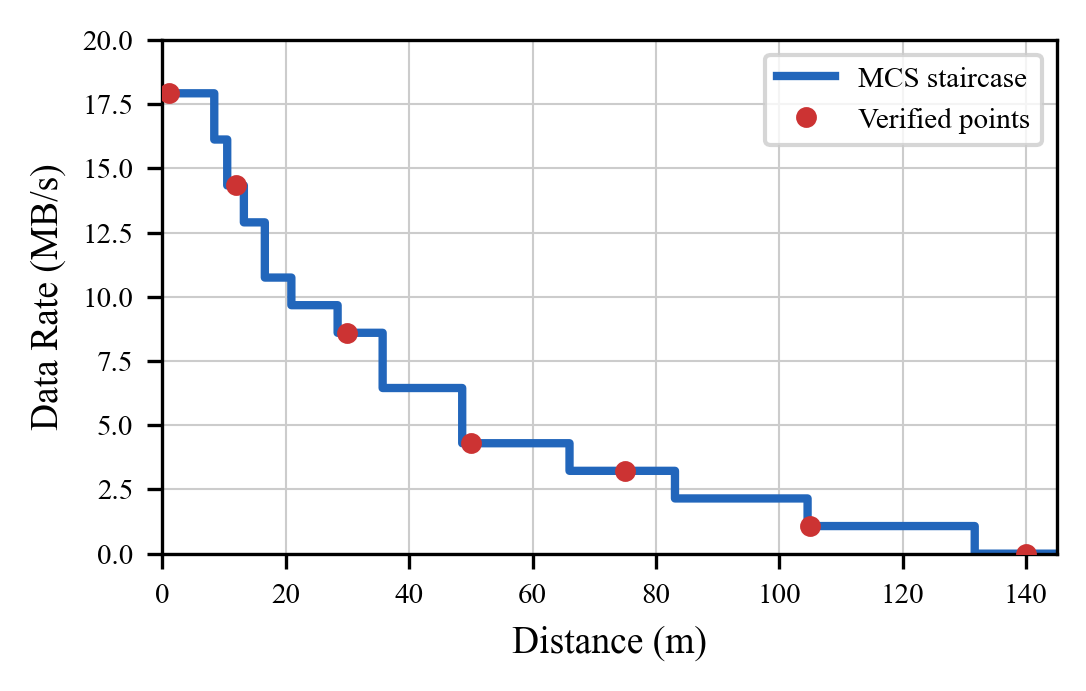
\includegraphics[width=\columnwidth]{figures/exp1_mcs_staircase.png}
\caption{Experiment 1: PHY data rate vs.\ link distance showing discrete MCS
  transitions (802.11ax, 5\,GHz, $n{=}3$).  Red dots mark experimentally
  verified data points from \Cref{tab:exp1}.}
\label{fig:exp1}
\end{figure}

\subsubsection{Experiment 2: Parallel Link Separation}

Two parallel 30\,m links separated vertically by distances from 5\,m to
200\,m.  \Cref{fig:exp2} illustrates the three interference regimes.
At separation $\leq 70$\,m, all node pairs are within the carrier
sensing range (71.2\,m), so the links \emph{contend} via Bianchi's model:
each gets $\eta(2)/2 \approx 0.44$ of the base rate 8.6\,MB/s $= 3.79$\,MB/s.
At separation $\geq 75$\,m, the links become hidden terminals, and SINR
degradation determines the effective rate.

Notably, the effective rate \emph{drops} at the CS range boundary: from
3.79\,MB/s (contention) to 3.23\,MB/s (hidden terminal at 75\,m), before
recovering at larger separations.  This non-monotonic behavior is the
classic \emph{hidden terminal effect}: within sensing range, links coordinate
via CSMA/CA and time-share the channel fairly (each receiving 44\% of the
full 8.6\,MB/s); just outside sensing range, links transmit simultaneously
without coordination, and the resulting mutual interference degrades each
receiver's SINR enough to force a lower MCS rate (from MCS~5 to MCS~2).
The hidden terminal regime is thus \emph{worse} than fair contention sharing
at close range.  As separation increases further, interference power
diminishes: SINR recovers to MCS~3 (4.3\,MB/s) at 90\,m and MCS~4
(6.45\,MB/s) at 130\,m.  All 15 data points match predictions exactly.

\begin{figure}[t]
\centering

\includegraphics[width=\columnwidth]{figures/exp2_parallel_separation.png}
\caption{Experiment 2: effective per-link rate vs.\ separation for two
  parallel 30\,m links.  The non-monotonic dip at the CS boundary
  (71.2\,m) is the hidden-terminal effect, analyzed in the body text.}
\label{fig:exp2}
\end{figure}

\subsubsection{Experiment 4: Three Parallel Links}

This experiment extends the two-link topology of Experiment~2 to three
parallel 30\,m links placed at $y = 0$, $y = s$, and $y = 2s$ (links A,
B, C), each carrying a 10\,MB transfer.  \Cref{fig:exp4_setup} illustrates
the topology with separation~$s$ as the independent variable.

\begin{figure}[t]
\centering
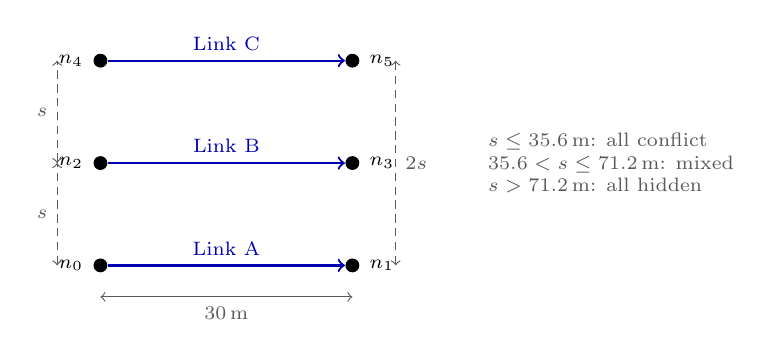
\begin{tikzpicture}[
  nd/.style={circle, fill=black, inner sep=0pt, minimum size=5pt},
  lnk/.style={->, thick, blue!70!black},
  sep/.style={<->, densely dashed, gray!70!black},
  annot/.style={font=\scriptsize, text=gray!70!black},
]
  % Link A (bottom)
  \node[nd, label={[font=\scriptsize]left:$n_0$}] (a0) at (0,0) {};
  \node[nd, label={[font=\scriptsize]right:$n_1$}] (a1) at (3.2,0) {};
  \draw[lnk] (a0) -- node[above, font=\scriptsize] {Link A} (a1);

  % Link B (middle)
  \node[nd, label={[font=\scriptsize]left:$n_2$}] (b0) at (0,1.3) {};
  \node[nd, label={[font=\scriptsize]right:$n_3$}] (b1) at (3.2,1.3) {};
  \draw[lnk] (b0) -- node[above, font=\scriptsize] {Link B} (b1);

  % Link C (top)
  \node[nd, label={[font=\scriptsize]left:$n_4$}] (c0) at (0,2.6) {};
  \node[nd, label={[font=\scriptsize]right:$n_5$}] (c1) at (3.2,2.6) {};
  \draw[lnk] (c0) -- node[above, font=\scriptsize] {Link C} (c1);

  % Separation arrows
  \draw[sep] (-0.55,0) -- node[left, annot] {$s$} (-0.55,1.3);
  \draw[sep] (-0.55,1.3) -- node[left, annot] {$s$} (-0.55,2.6);

  % A-C distance
  \draw[sep] (3.75,0) -- node[right, annot] {$2s$} (3.75,2.6);

  % Link length
  \draw[<->, gray!70!black] (0,-0.4) -- node[below, annot] {30\,m} (3.2,-0.4);

  % Regime annotations (right side)
  \node[annot, align=left, anchor=west] at (4.8,1.3) {%
    $s \leq 35.6$\,m: all conflict\\
    $35.6 < s \leq 71.2$\,m: mixed\\
    $s > 71.2$\,m: all hidden};
\end{tikzpicture}
\caption{Experiment~4 topology: three parallel 30\,m links at variable
  separation~$s$.  As $s$ increases, the interference regime transitions
  from all-conflict to mixed (adjacent pairs contend, outer pair A--C
  are hidden terminals) to all-hidden.}
\label{fig:exp4_setup}
\end{figure}

As $s$ increases, three interference regimes emerge: (i)~\emph{all-conflict}
($s \leq 35.6\,$m): all three pairs are within $d_{\text{CS}}$, each link
gets $R_{\text{base}} \cdot \eta(3)/3$; (ii)~\emph{mixed}
($35.6 < s \leq 71.2\,$m): adjacent pairs (A--B, B--C) contend via
Bianchi, while the outer pair (A--C at distance~$2s$) are hidden terminals,
creating asymmetric rates; and (iii)~\emph{all-hidden} ($s > 71.2\,$m):
no conflict-graph edges, each link sees the others purely as hidden
terminals.  Because A/C and B generally have different rates, one group
finishes first, and the remaining links' interference conditions change.
The analytical prediction accounts for this multi-phase behavior.

\begin{table}[t]
\centering
\caption{Experiment~4: Three parallel links at varying separation.
  In the mixed regime the middle link~B contends with both neighbors
  while outer links A, C contend only with B and see each other as
  hidden terminals.}
\label{tab:exp4}
\begin{tabular}{@{}rlrrrr@{}}
\toprule
$s$(m) & Regime & Pred $R_A$ & Sim $R_A$ & Pred $R_B$ & Sim $R_B$ \\
\midrule
10  & all-conf & 2.461 & 2.461 & 2.461 & 2.461 \\
35  & all-conf & 2.461 & 2.461 & 2.461 & 2.461 \\
40  & mixed    & 1.861 & 1.861 & 2.461 & 2.461 \\
50  & mixed    & 2.174 & 2.174 & 2.461 & 2.461 \\
70  & mixed    & 2.840 & 2.840 & 2.720 & 2.720 \\
75  & all-hid  & 3.225 & 3.225 & 2.867 & 2.867 \\
100 & all-hid  & 4.300 & 4.300 & 3.822 & 3.822 \\
150 & all-hid  & 6.450 & 6.450 & 5.160 & 5.160 \\
\bottomrule
\multicolumn{6}{@{}l}{\scriptsize A$=$C by symmetry in all cases.  Rates in MB/s.}
\end{tabular}
\end{table}

\Cref{tab:exp4} shows the results.  All 11 test points match exactly.
In the mixed regime at $s{=}70\,$m, an interesting crossover occurs where
A/C become faster than B, because the outer links benefit from their
mutual hidden-terminal distance while B contends with both neighbors.
This experiment validates the model's ability to correctly compose
Bianchi contention and SINR degradation in a single topology with
asymmetric interference conditions and multi-phase dynamic recalculation.

\subsubsection{Additional Validation Experiments}

Five additional experiments validate: (3)~two-transmitter shared-receiver
topologies, (5)~staggered transfer starts with dynamic
recalculation, (6)~per-link bandwidth sharing with multiple flows,
(8)~five-link hidden terminal cascades with different data sizes, and
(9)~combined bandwidth sharing with hidden terminal interference.  All pass.


\subsection{External Validation Against Bianchi (2000)}
\label{sec:external_val}

Internal validation confirms self-consistency but does not establish
that our implementation of Bianchi's equations is correct.  We therefore
reproduce the numerical results from Bianchi's original paper
\cite{bianchi2000} using his exact parameters: FHSS 1\,Mbps basic
access (no RTS/CTS), with slot duration 50\,$\mu$s, SIFS 28\,$\mu$s,
DIFS 128\,$\mu$s, propagation delay 1\,$\mu$s, payload 8184 bits,
MAC header 272 bits, PHY header 128 bits, and ACK 112 bits.

\subsubsection{Table III Reproduction}

\Cref{tab:bianchi_table3} compares our computed normalized saturation
throughput $S$ against the values published in Bianchi's Table~III for
$W{=}32$, $m{=}3$.  At $n{=}2$, our solver computes $S = 0.847311$
versus the published $0.8473$ (relative error $0.001\%$).  At $n{=}3$,
we compute $S = 0.836828$ versus $0.8368$ (relative error $0.003\%$).
These sub-basis-point differences are consistent with rounding in the
published table.

\begin{table}[t]
\centering
\caption{Reproduction of Bianchi~\cite{bianchi2000} Table~III:
normalized saturation throughput $S$ for $W{=}32$, $m{=}3$.}
\label{tab:bianchi_table3}
\begin{tabular}{@{}rrrr@{}}
\toprule
$n$ & \textbf{Computed} & \textbf{Published} & \textbf{Rel.\ Error} \\
\midrule
2  & 0.847311 & 0.8473 & 0.001\% \\
3  & 0.836828 & 0.8368 & 0.003\% \\
\bottomrule
\end{tabular}
\end{table}

We solve the coupled equations (\Cref{eq:tau,eq:p}) by bisection rather
than fixed-point iteration, which can oscillate when the mapping slope
exceeds unity; with $\epsilon = 10^{-12}$ convergence is guaranteed in
at most 40 steps.

\subsubsection{Figure 6 Reproduction}

\Cref{fig:bianchi_fig6} reproduces Bianchi's Figure~6 throughput curves
for $W{=}32$, $m{=}5$ and $W{=}128$, $m{=}3$ across $n{=}5$ to $n{=}50$
stations.  Both curves match the expected monotonic throughput decay;
the $W{=}128$ curve reproduces the slight non-monotonicity between
$n{=}5$ and $n{=}10$ consistent with Bianchi's published results.
Data points digitized from Bianchi's original figure overlay our
computed curves to within 0.34\% relative error.

\begin{figure}[t]
\centering

\includegraphics[width=\columnwidth]{figures/bianchi_fig6_overlay.png}
\caption{Reproduction of Bianchi~\cite{bianchi2000} Figure~6:
  normalized saturation throughput vs.\ number of stations for two
  $(W, m)$ configurations.  The $W{=}128$ curve's non-monotonicity
  between $n{=}5$ and $n{=}10$ is consistent with Bianchi's published
  results.  Digitized data points overlay our curves to within 0.34\%
  relative error, confirming faithful reproduction.}
\label{fig:bianchi_fig6}
\end{figure}

\subsubsection{N-Way Contention Scaling}

To confirm that the Bianchi model scales correctly within the full
simulation loop, we place $n \in \{2, \ldots, 8\}$ parallel 30\,m links
at 5\,m separation (all within carrier-sensing range), each carrying a
10\,MB transfer.

\begin{table}[t]
\centering
\caption{N-way Bianchi contention scaling (30\,m links at 5\,m
separation).  $\eta(n)$ is the Bianchi MAC efficiency.}
\label{tab:exp7}
\begin{tabular}{@{}rrrrrr@{}}
\toprule
$n$ & $\eta(n)$ & $\eta(n)/n$ & \textbf{Pred(MB/s)} & \textbf{Sim(MB/s)} \\
\midrule
2 & 0.881 & 0.440 & 3.787 & 3.787 \\
3 & 0.859 & 0.286 & 2.461 & 2.461 \\
4 & 0.837 & 0.209 & 1.799 & 1.799 \\
5 & 0.818 & 0.164 & 1.407 & 1.407 \\
6 & 0.802 & 0.134 & 1.149 & 1.149 \\
7 & 0.788 & 0.113 & 0.968 & 0.968 \\
8 & 0.726 & 0.091 & 0.780 & 0.780 \\
\bottomrule
\end{tabular}
\end{table}

\Cref{tab:exp7} confirms the Bianchi solver produces correct throughput
predictions when embedded in the full simulation engine with real RF
parameters and dynamic recalculation.


\subsection{Cross-Validation Against ns-3}
\label{sec:ns3_validation}

Rungs~1 and~2 establish internal self-consistency and faithful
reproduction of Bianchi's analytical framework, but all comparisons are
against formulas \ncsim{} itself implements.  Rung~3 cross-validates the
\emph{combined} model (path loss + MCS selection + CSMA/CA + hidden
terminal capture) against ns-3~\cite{ns3}, a packet-level simulator
that models 802.11 at full protocol fidelity.

Both experiments use 802.11ax at 5\,GHz on a 20\,MHz channel with
parameters matched between ncsim's \texttt{RFConfig} defaults and ns-3's
\texttt{ConstantRateWifiManager} (see \Cref{tab:ns3_params} for the full
list).  Critically, A-MPDU is disabled to match Bianchi's single-frame
assumption.  Each ns-3 point is the mean over 20 seeds (30\,s per run,
first 2\,s discarded as warmup).

\subsubsection{Experiment 1: Contention Scaling}

We place $n \in \{1, \ldots, 8\}$ co-located STA-AP link pairs at 30\,m
link length and 5\,m vertical separation, all well within the 71.2\,m
carrier-sensing range, creating a complete conflict graph.  Each STA sends
saturated UDP traffic to its AP.  \Cref{fig:ns3_validation}(a) overlays
\ncsim{}'s Bianchi prediction $R_{\text{base}} \cdot \eta(n)/n$ against the
ns-3 per-station goodput.

\ncsim{}'s Bianchi model, which accounts for PHY overhead (preamble, SIFS,
ACK) in the efficiency computation, tracks ns-3 closely across all station
counts.  At $n{=}1$, the solo goodput predictions differ by only 0.3\%
(3.78 vs.\ 3.77\,MB/s).  The maximum error of 7.6\% occurs at $n{=}7$,
where the Bianchi fixed-point approximation slightly overestimates MAC
efficiency.  The mean error across all $n$ is 4.0\%.  Both curves exhibit
the same monotonic decay shape with Pearson correlation $r > 0.999$.  All
95\% confidence intervals are below $\pm 0.02$\,MB/s, confirming that
30\,s of saturated traffic reaches steady state.

\subsubsection{Experiment 2: Separation Sweep}

Two parallel 30\,m links are placed at vertical separation
$s \in \{10, 20, \ldots, 200\}$\,m.  As $s$ increases beyond the 71.2\,m
carrier-sensing boundary, the links transition from Bianchi contention
(symmetric time-sharing at $\eta(2)/2$) to the hidden terminal regime,
where simultaneous transmissions may corrupt frames at the receiver.
\ncsim{}'s capture-threshold model (\Cref{eq:capture}) predicts a
\emph{throughput dip} at the CS boundary: per-link rate drops from
1.94\,MB/s (contention) to 1.50\,MB/s (hidden terminal frame loss) before
recovering sharply at $s = 120$\,m when the interferer's power falls below
the capture threshold and frames are decoded successfully at the full solo
rate (3.78\,MB/s).  \Cref{fig:ns3_validation}(b) overlays ns-3 results.

ns-3 confirms the qualitative behavior across all regimes.
In the contention zone ($s \leq 70$\,m), ns-3 goodput is stable at
1.92--2.06\,MB/s (1--6\% from \ncsim{}).  At the CS boundary
($s = 72$\,m), ns-3 exhibits a throughput dip to 1.34\,MB/s, confirming
\ncsim{}'s predicted dip direction and location (11\% error).  In the
hidden terminal zone ($s = 72$--$100$\,m), \ncsim{}'s capture-threshold
model predicts 1.50\,MB/s and ns-3 measures 1.34--1.50\,MB/s (0.5--11\%
error).  At large separations ($s \geq 120$\,m) where interference
power falls below the capture threshold, both models show recovery:
\ncsim{} predicts the full solo rate of 3.78\,MB/s and ns-3 reaches
3.62--3.77\,MB/s (0.3--4.4\% error).

\begin{figure}[t]
\centering

\includegraphics[width=\columnwidth]{figures/ns3_validation.png}
\caption{Cross-validation of \ncsim{} against ns-3.  (a)~$n$-way
  saturated goodput; (b)~two-link throughput vs.\ separation.  \ncsim{}
  tracks ns-3 within 0.3--11\% across all regimes.  Parameters
  per \Cref{tab:ns3_params}; each ns-3 point: mean $\pm$ 95\% CI over
  20 seeds.}
\label{fig:ns3_validation}
\end{figure}

\begin{table}[t]
\centering
\caption{Aligned parameters for ns-3 cross-validation.}
\label{tab:ns3_params}
\begin{tabular}{@{}lll@{}}
\toprule
\textbf{Parameter} & \textbf{ncsim} & \textbf{ns-3} \\
\midrule
TX power & 20\,dBm & \texttt{TxPowerStart/End = 20} \\
Frequency & 5\,GHz & Band 5\,GHz, ch.\,36 \\
Channel width & 20\,MHz & \texttt{ChannelSettings} \\
Path loss exp. & 3.0 & \texttt{Exponent = 3.0} \\
Ref.\ loss (1\,m) & 46.4\,dB & \texttt{ReferenceLoss = 46.4} \\
Noise floor & $-95$\,dBm & \texttt{RxNoiseFigure = 6} \\
CCA threshold & $-82$\,dBm & \texttt{CcaEdThreshold = -82} \\
CW$_{\min}$ & 16 & \texttt{MinCw = 15} \\
CW$_{\max}$ & 1024 & \texttt{MaxCw = 1023} \\
A-MPDU & disabled & \texttt{MaxAmpduSize = 0} \\
Guard interval & 3200\,ns & \texttt{GuardInterval = 3200} \\
\bottomrule
\end{tabular}
\end{table}

The ns-3 simulation scripts, Dockerfile for reproducible builds, and all
raw results are included in the paper's supplementary repository under
\texttt{paper/ns3/}.


%% ============================================================
\section{Experimental Evaluation}
\label{sec:eval}

The central finding of this paper is that interference-free evaluation
produces wrong scheduler rankings in over a quarter of scenarios tested.
The four subsections that follow build the evidence progressively:
routing interactions with interference (\Cref{sec:routing_eval}),
magnitude of interference impact (\Cref{sec:interference_eval}),
rank inversions in a 108-run factorial (\Cref{sec:scheduler_eval}),
and sensitivity analyses delineating an \emph{interference danger
zone}, the parameter regimes where interference is most consequential
(\Cref{sec:sensitivity}).

All experiments use 802.11ax at 5\,GHz with a path loss exponent of
$n = 3$ (except where explicitly varied), heterogeneous compute capacities
(80--300 units/s), 10\,MB data payloads per DAG edge, and deterministic
seed~42.

Three DAG structures of increasing complexity are used across all
experiments:
\begin{itemize}[itemsep=1pt,leftmargin=*]
\item \textbf{Small (5 tasks):} Fork-join, $T_0 \to \{T_1, T_2, T_3\}
  \to T_4$.
\item \textbf{Medium (10 tasks):} Diamond, $T_0 \to \{T_1\text{--}T_4\}
  \to \{T_5\text{--}T_8\} \to T_9$ with selective cross-links between
  layers.
\item \textbf{Large (20 tasks):} Multi-level pipeline, $T_0 \to 4 \to 6
  \to 6 \to 3$ tasks per layer with sparse inter-layer connections.
\end{itemize}
\noindent All tasks have \texttt{compute\_cost}${}= 500$ and all edges have
\texttt{data\_size}${}= 10$\,MB (except where varied in
\Cref{sec:sensitivity}).

\subsection{Scheduler Information and Fairness}
\label{sec:scheduler_info}

Both the interference-free and interference-aware modes present an
identical \texttt{NetworkSnapshot} to the scheduler, containing the same
WiFi-derived link bandwidths (\Cref{tab:scheduler_info}).  No scheduler
sees the conflict graph or contention factors; these are runtime phenomena
computed \emph{after} the schedule has been committed.  Any difference
in makespan is therefore attributable solely to interference that the
scheduler could not anticipate.

\begin{table}[t]
\centering
\caption{Scheduler inputs.  No scheduler observes interference.}
\label{tab:scheduler_info}
\setlength{\tabcolsep}{3pt}
\begin{tabular}{@{}llll@{}}
\toprule
\textbf{Scheduler} & \textbf{Planner Inputs} &
  \textbf{Network View} & \textbf{Intf?} \\
\midrule
Manual     & Pin annotations      & N/A                & No \\
RoundRobin & Node list            & N/A                & No \\
HEFT       & DAG, $C_v$, $B_\ell$ & Full virtual net$^\dagger$ & No \\
CPOP       & DAG, $C_v$, $B_\ell$ & Full virtual net$^\dagger$ & No \\
\bottomrule
\multicolumn{4}{@{}l}{\scriptsize $^\dagger$Actual BW for reachable pairs;
  0.001\,MB/s for unreachable.}
\end{tabular}
\end{table}

\subsection{Routing Strategy Comparison}
\label{sec:routing_eval}

Because multi-hop routing determines contention domains, we first
establish how routing strategies interact with interference before
evaluating schedulers.  We compare widest-path and shortest-path routing
under HEFT scheduling with the interference-aware model across grid mesh
networks of three sizes (2$\times$2, 3$\times$3, 4$\times$4) and three
DAG complexities (5, 10, and 20 tasks).  All links use 40\,m grid
spacing with heterogeneous compute capacities (80--300 units/s).

\Cref{fig:routing-topo} shows the resulting link utilization for each strategy.
Link color and thickness indicate the number of bidirectional data flows
traversing each link.  Widest-path routing funnels nearly all traffic through
an 8-hop perimeter corridor (nodes 0--1--2--6--10--14--13--12), loading each
link with 9--10 flows and leaving the right half of the network idle.
Shortest-path routing distributes traffic across 12 links with shorter routes
(avg 3.1 hops vs.\ 4.5), spreading load more evenly.  Under CSMA contention,
widest-path's flow concentration produces severe airtime competition: its
makespan is 1341\,s compared to 712\,s for shortest-path (1.9$\times$ slower).
The result illustrates that single-flow optimal routing (maximizing bottleneck
bandwidth) becomes counterproductive when multiple concurrent transfers compete
for shared wireless airtime.

\begin{figure}[t]
\centering

\includegraphics[width=\columnwidth]{figures/routing_topo_4x4_largedag.png}
\caption{Link utilization under widest-path (left) vs.\ shortest-path (right)
  routing on a 4$\times$4 grid mesh with a 20-task DAG.  Widest-path
  concentrates 9--10 flows on an 8-hop perimeter corridor; shortest-path
  spreads traffic across 12 links with shorter routes, reducing makespan by
  1.9$\times$ under CSMA contention.}
\label{fig:routing-topo}
\end{figure}

\begin{table}[t]
\centering
\caption{Routing comparison: makespan (seconds) for widest-path (W) vs.\
shortest-path (S) under HEFT with \texttt{csma\_bianchi}.}
\label{tab:routing}
\begin{tabular}{@{}llrrr@{}}
\toprule
\textbf{Network} & \textbf{DAG} & \textbf{W (s)} & \textbf{S (s)} & \textbf{Winner} \\
\midrule
\multirow{3}{*}{2$\times$2 (4 nodes)}
  & 5 tasks   & 15.38  & 15.38  & Tie \\
  & 10 tasks  & 32.60  & 32.50  & Shortest \\
  & 20 tasks  & 88.13  & 64.51  & Shortest \\
\midrule
\multirow{3}{*}{3$\times$3 (9 nodes)}
  & 5 tasks   & 19.06  & 19.06  & Tie \\
  & 10 tasks  & 79.88  & 35.16  & Shortest \\
  & 20 tasks  & 142.94 & 96.70  & Shortest \\
\midrule
\multirow{3}{*}{4$\times$4 (16 nodes)}
  & 5 tasks   & 315.20 & 12.88  & Shortest \\
  & 10 tasks  & 1396.9 & 827.23 & Shortest \\
  & 20 tasks  & 1703.4 & 794.39 & Shortest \\
\bottomrule
\end{tabular}
\end{table}

\textbf{Key findings.}
Shortest-path routing wins in 7 of 9 configurations with 2 ties.  The
advantage is most pronounced in the 4$\times$4 grid, where widest-path
routing selects longer paths with higher bottleneck bandwidth but incurs
substantially more wireless interference due to multi-hop transmissions
traversing more contention domains.  In the 4$\times$4 grid with 5 tasks,
widest-path achieves a makespan of 315.2\,s compared to 12.9\,s for
shortest-path, a $24\times$ difference, because the widest paths route
transfers through 3--4 hops across the full grid diameter, creating
overlapping contention domains that reduce effective bandwidth to a
fraction of the solo rate.


\subsection{Interference Impact Analysis}
\label{sec:interference_eval}

Before asking whether interference changes scheduler \emph{rankings},
we first quantify whether it changes absolute makespans enough to
matter.  We measure the impact of CSMA/CA interference by running each
of the nine grid-network scenarios with the interference-aware model
versus the interference-free model, both using shortest-path routing
and HEFT.  As detailed in \Cref{sec:scheduler_info}, both modes
present identical \texttt{NetworkSnapshot} inputs to the scheduler;
the only difference is the presence or absence of runtime contention
and hidden-terminal effects.  \Cref{tab:interference} shows slowdowns
ranging from 35\% to 5{,}406\%, large enough that the
interference-free model is objectively unreliable for scheduler
selection in these regimes.

\begin{table}[t]
\centering
\caption{Interference impact: makespan (seconds) without interference vs.\
with \texttt{csma\_bianchi}, using shortest-path routing.  HEFT and CPOP
produce identical placements on the 5-task DAG but diverge as DAG
complexity grows.}
\label{tab:interference}
\setlength{\tabcolsep}{2.5pt}
\begin{tabular}{@{}ll|rrr|rrr@{}}
\toprule
& & \multicolumn{3}{c|}{\textbf{HEFT}} & \multicolumn{3}{c}{\textbf{CPOP}} \\
\textbf{Net.} & \textbf{DAG} &
  \textbf{None} & \textbf{Bian.} & \textbf{Slow.} &
  \textbf{None} & \textbf{Bian.} & \textbf{Slow.} \\
\midrule
\multirow{3}{*}{2$\times$2}
  & 5T  & 11.43 & 15.38 & +35\%   & 11.43 & 15.38 & +35\%   \\
  & 10T & 18.76 & 32.50 & +73\%   & 18.76 & 41.32 & +120\%  \\
  & 20T & 27.50 & 64.51 & +135\%  & 29.53 & 70.96 & +140\%  \\
\midrule
\multirow{3}{*}{3$\times$3}
  & 5T  & 8.43  & 19.06 & +126\%  & 8.43  & 19.06 & +126\%  \\
  & 10T & 12.76 & 35.16 & +176\%  & 13.65 & 52.01 & +281\%  \\
  & 20T & 17.11 & 96.70 & +465\%  & 19.98 & 104.24 & +422\% \\
\midrule
\multirow{3}{*}{4$\times$4}
  & 5T  & 8.93  & 12.88 & +44\%    & 8.93  & 12.88 & +44\%    \\
  & 10T & 15.02 & 827.23 & +5406\% & 15.02 & 827.23 & +5406\% \\
  & 20T & 21.75 & 794.39 & +3553\% & 20.65 & 873.26 & +4129\% \\
\bottomrule
\end{tabular}
\end{table}

\textbf{Key findings.}
Interference impact ranges from 35\% to over 5400\% across all
configurations.  Several patterns emerge:

\begin{itemize}[itemsep=1pt,leftmargin=*]
\item \textbf{No configuration escapes contention entirely.}  Even the
  smallest scenario (2$\times$2, 5 tasks) shows a 35\% slowdown, because
  the Bianchi MAC overhead reduces effective throughput whenever links
  share the channel.
\item \textbf{Denser networks amplify interference.}  The 3$\times$3 grid
  (32 links) shows 126--465\% slowdown, while the 4$\times$4 grid (68 links)
  shows up to 5406\%.  More links create larger conflict neighborhoods.
\item \textbf{Dense interference creates cascading delays.}  In the
  4$\times$4 grid, HEFT distributes tasks across 16 nodes assuming
  uncontested bandwidth.  During execution, many simultaneous transfers
  contend, reducing effective rates and causing HEFT's schedule to
  become severely suboptimal.
\item \textbf{CPOP shows equal or worse slowdowns.}  CPOP matches HEFT
  on the 5-task DAG (identical placements), but exhibits higher slowdowns
  on larger DAGs in the 2$\times$2 and 3$\times$3 grids (e.g., 281\%
  vs.\ 176\% for 10 tasks on 3$\times$3).  CPOP's critical-path-based
  allocation concentrates communication along fewer paths, making those
  paths more vulnerable to contention.  In the 4$\times$4 grid, both
  schedulers suffer extreme slowdowns.
\end{itemize}

\noindent These results demonstrate that ignoring wireless interference in
scheduling can lead to order-of-magnitude performance prediction errors,
motivating the physically-grounded model in \ncsim{}.


\subsection{Scheduler Comparison and Rank Inversions}
\label{sec:scheduler_eval}

The interference impact results above suggest a deeper question: does
ignoring interference merely produce inaccurate makespan predictions, or
does it lead to wrong \emph{choices} among schedulers?  To answer this, we
execute a full factorial comparison: 3 networks $\times$ 3 DAGs $\times$
3 schedulers (HEFT, CPOP, RoundRobin) $\times$ 2 routings $\times$ 2
interference models $= 108$ simulation runs.  All runs use 802.11ax at
5\,GHz, heterogeneous compute capacities, and seed~42.

For each of the 18 (network, DAG, routing) triples, we identify the best
scheduler under each interference model.  A \emph{rank inversion} occurs
when the winning scheduler changes between the interference-free and
interference-aware models.  The \emph{scheduling regret} is the relative
performance penalty from deploying the interference-free-optimal scheduler
in the presence of interference.

\Cref{tab:winner_matrix} presents makespan ratios for each scheduler
relative to the best under the interference-aware model; a ratio of 1.00 denotes the
optimal choice.  The key statistics are:
\begin{itemize}[itemsep=1pt,leftmargin=*]
\item \textbf{Rank inversion rate: 27.8\%} (5 of 18 triples).
\item \textbf{Mean relative regret: 20.2\%} across all 18 triples.
\item \textbf{Maximum relative regret: 168.3\%} ($4\times4$ grid,
  10-task DAG, widest-path: HEFT chosen under the interference-free
  model gives 1396.9\,s, but round-robin achieves 520.6\,s under the
  interference-aware model).
\end{itemize}

\begin{table*}[t]
\centering
\caption{Makespan ratios under \texttt{csma\_bianchi} relative to the best
  scheduler for each (network, DAG, routing) triple.  A ratio of 1.00
  denotes the optimal choice; higher values show how much worse that
  scheduler performs.  ``None$\downarrow$'' indicates which scheduler an
  interference-free evaluation would select.  Bold entries mark rank
  inversions where the interference-free choice is suboptimal.}
\label{tab:winner_matrix}
\setlength{\tabcolsep}{3.5pt}
\begin{tabular}{@{}ll|rrrl|rrrl@{}}
\toprule
& & \multicolumn{4}{c|}{\textbf{Widest-path}} &
  \multicolumn{4}{c}{\textbf{Shortest-path}} \\
\textbf{Net.} & \textbf{DAG} &
  \textbf{H} & \textbf{C} & \textbf{RR} & \textbf{None$\downarrow$} &
  \textbf{H} & \textbf{C} & \textbf{RR} & \textbf{None$\downarrow$} \\
\midrule
\multirow{3}{*}{$2\times2$}
  & 5T  & 1.00 & 1.00 & 2.71 & HEFT & 1.00 & 1.00 & 2.01 & HEFT \\
  & 10T & 1.00 & 1.52 & 2.38 & HEFT & 1.00 & 1.27 & 1.74 & HEFT \\
  & 20T & 1.13 & 1.00 & 1.63 & CPOP & 1.00 & 1.10 & 1.69 & HEFT \\
\midrule
\multirow{3}{*}{$3\times3$}
  & 5T  & 1.00 & 1.00 & 2.00 & HEFT & 1.00 & 1.00 & 2.00 & HEFT \\
  & 10T & 1.19 & 1.00 & 8.32 & CPOP & 1.00 & 1.48 & 13.05 & HEFT \\
  & 20T & 1.00 & 1.79 & 6.49 & HEFT & 1.00 & 1.08 & 8.31 & HEFT \\
\midrule
\multirow{3}{*}{$4\times4$}
  & 5T  & 1.60 & 1.60 & 1.00 & \textbf{HEFT} & 1.00 & 1.00 & 6.56 & HEFT \\
  & 10T & 2.68 & 2.68 & 1.00 & \textbf{HEFT} & 1.98 & 1.98 & 1.00 & \textbf{HEFT} \\
  & 20T & 1.01 & 1.28 & 1.00 & \textbf{CPOP} & 1.00 & 1.10 & 1.97 & \textbf{CPOP} \\
\bottomrule
\end{tabular}
\end{table*}

\textbf{HEFT dominates under interference-free models.}  Under the
interference-free model, HEFT or CPOP wins in all 18 triples.  This
is expected: both algorithms optimize the critical path by distributing
tasks across nodes to maximize parallelism, assuming uncontested bandwidth.
The sophisticated scheduling logic of HEFT and CPOP provides clear
advantages when the network behaves as these algorithms assume it will.

\textbf{Round-robin wins in large networks under interference.}
In the $4\times4$ grid with the interference-aware model and widest-path routing,
round-robin wins for all three DAG sizes, a striking reversal.  The
mechanism is clear: HEFT spreads tasks across many of the 16 available
nodes to exploit parallelism, but this creates many concurrent multi-hop
transfers that contend on shared wireless channels.  Round-robin's simpler
placement cycles through nodes in order, which tends to concentrate work
on nearby nodes with fewer concurrent transfers and thus less contention.

To illustrate this mechanism concretely, consider the most dramatic rank
inversion: the $4\times4$ grid with 10 tasks and widest-path routing.
Under the interference-free model, HEFT achieves a makespan of 14.9\,s by
distributing tasks across many of the 16 nodes, creating multiple concurrent
inter-node transfers that exploit the assumed link bandwidths.  However,
under the interference-aware model, these concurrent transfers contend on overlapping
conflict graph neighborhoods: each transfer's effective bandwidth drops to
a fraction of its solo rate as the Bianchi model allocates channel time
among contenders.  The resulting makespan increases to
1,396.9\,s, a $94\times$ blowup.  In contrast, round-robin achieves
520.6\,s under the same interference model.  Although round-robin makes no
attempt to optimize the critical path, its placement pattern generates fewer
concurrent transfers, resulting in less severe contention.  The scheduling
regret, the penalty for choosing HEFT based on the interference-free
evaluation, is 168\%.  A researcher evaluating these schedulers without
interference modeling would confidently select HEFT, unaware that it
produces $2.7\times$ worse performance than a round-robin
baseline.

\textbf{Routing modulates the effect.}  Shortest-path routing mitigates
rank inversions in some cases by reducing the number of hops per transfer
and thus the number of contention domains traversed.  The $4\times4$ /
5-task scenario shows a rank inversion under widest-path routing (60\%
regret) but not under shortest-path (zero regret).  However, shortest-path
does not eliminate inversions entirely: in the $4\times4$ / 10-task
scenario, the inversion persists even with shortest-path routing (98\%
regret), because the DAG is large enough to generate concurrent transfers
even along short paths.

\Cref{fig:regret_scatter} visualizes the regret ratio (naive makespan
divided by oracle makespan) for all 18 triples.  The 13 triples at 1.0
show zero regret; the 5 bars above 1.0 are rank inversions, with the
$4\times4$ / 10-task / widest-path case reaching $2.68\times$.

\begin{figure}[t]
\centering

\includegraphics[width=\columnwidth]{figures/regret_scatter.png}
\caption{Scheduling regret ratios.  Each bar shows the ratio of the
  interference-free-optimal makespan (scheduler chosen under the
  interference-free model, run under the interference-aware model) to
  the oracle makespan (best scheduler under interference).  A ratio
  of 1.0 indicates zero regret; red bars mark rank inversions where
  the interference-free choice is suboptimal.}
\label{fig:regret_scatter}
\end{figure}

These results demonstrate a key capability of \ncsim{}: by jointly modeling
scheduling and wireless interference, it reveals that interference-free
evaluations can lead to
systematically wrong policy choices, a finding that would be invisible to
tools that abstract away wireless contention.


\subsection{Sensitivity Analysis}
\label{sec:sensitivity}

The results above demonstrate that wireless interference can dramatically
affect scheduler rankings.  However, a natural question arises: under what
conditions is interference most consequential, and when can it safely be
ignored?  To address this question, we conduct two sensitivity sweeps
that vary key parameters affecting interference severity: the
communication-to-computation ratio (data size per DAG edge) and the level
of concurrent workload (number of simultaneous DAGs).

\subsubsection{Communication-to-Computation Ratio}

The communication-to-computation ratio (CCR) determines the relative
importance of network transfer time versus compute time.  We sweep data
size per edge across $\{1, 2, 5, 10, 20, 50, 100\}$\,MB on the 3$\times$3
grid with HEFT and shortest-path routing, testing all three DAG types
(5, 10, and 20 tasks).  \Cref{fig:ccr} shows the interference slowdown
as a function of CCR.

The results reveal a non-monotonic pattern: slowdown peaks at intermediate
CCR values (${\approx}0.3$--$1.1$) and decreases at both extremes.  The
mechanism differs at each end.  At low CCR (1--2\,MB), transfers complete
so quickly that the probability of temporal overlap between concurrent
flows is small, and contention has little opportunity to develop.  At very
high CCR (50--100\,MB), HEFT's scheduling logic recognizes the enormous
transfer costs and collapses tasks onto fewer nodes to avoid inter-node
communication entirely, a scheduling adaptation that eliminates contention
by eliminating transfers.  The interference ``danger zone'' lies in
between, where transfers are long enough to overlap but the scheduler
still distributes tasks across multiple nodes.  For the 20-task DAG, the
peak slowdown of $7.3\times$ occurs at 10\,MB per edge, corresponding to
a CCR of approximately 0.5 (where transfer time and compute time are
comparable).

\begin{figure}[t]
\centering

\includegraphics[width=\columnwidth]{figures/sensitivity_ccr.png}
\caption{Interference slowdown vs.\ CCR (3$\times$3 grid,
  HEFT, shortest-path).  Slowdown peaks at intermediate CCR values
  where transfers are long enough to contend but not so large that the
  scheduler collapses tasks onto one node.  The 20-task DAG reaches
  $7.3\times$ at CCR$\approx 0.53$.}
\label{fig:ccr}
\end{figure}

\subsubsection{Multi-DAG Contention}

In practice, edge computing platforms rarely service a single workflow in
isolation; multiple applications submit DAGs concurrently, and their
transfers share the same wireless medium.  To evaluate how \ncsim{}
captures this multi-tenant scenario, we inject $k \in \{1, 2, 3, 4, 5\}$
identical 5-task fork-join DAGs with 0.5\,s stagger on the 3$\times$3 grid
(HEFT, shortest-path).  Each DAG is scheduled independently, meaning that
HEFT optimizes each workflow without knowledge of the others' transfers.

\Cref{fig:multidag} shows that contention scaling is super-linear
under \texttt{csma\_bianchi}.  Without interference, $k{=}5$ DAGs
produce $2.14\times$ the makespan of $k{=}1$ ($18.0$\,s vs.\ $8.4$\,s),
reflecting the expected linear increase from staggered injection plus
queuing at compute nodes.  With interference, however, $k{=}5$ produces
$3.86\times$ the single-DAG makespan ($73.5$\,s vs.\ $19.1$\,s).  The
gap between the two curves widens with each additional DAG: the slowdown
factor grows from $2.26\times$ at $k{=}1$ to $2.98\times$ at $k{=}2$ to
$4.08\times$ at $k{=}5$, indicating a positive feedback loop.  Each
additional DAG contributes its own transfers to the contention pool
and prolongs the duration of existing transfers (through reduced
effective bandwidth), which in turn increases the temporal overlap
with subsequent DAGs.  This super-linear scaling is invisible to
interference-free models, which predict near-linear growth and would
substantially underestimate the makespan of multi-tenant edge deployments.

\begin{figure}[t]
\centering

\includegraphics[width=\columnwidth]{figures/multidag.png}
\caption{Multi-DAG makespan scaling on 3$\times$3 grid (5-task DAGs,
  HEFT, shortest-path).  Contention amplifies super-linearly: the
  gap between the curves widens from $2.26\times$ ($k{=}1$) to
  $4.08\times$ ($k{=}5$).}
\label{fig:multidag}
\end{figure}

\subsubsection{Sensitivity Summary}

\Cref{tab:sensitivity_summary} consolidates the findings across both
sensitivity dimensions.  Taken together, these results delineate an
\emph{interference danger zone}, the conjunction of parameter settings
under which interference effects are most severe and most likely to change
scheduling conclusions.  Wireless interference has the greatest
impact, and is most likely to produce rank inversions, at moderate
communication-to-computation ratios (5--20\,MB payloads per edge) with
multiple concurrent workflows ($k \geq 2$).

These conditions are not exotic.  Data payloads of 5--20\,MB per DAG edge
are representative of computer vision pipelines (transferring image frames
between processing stages) and sensor fusion applications (aggregating data
from multiple modalities).  Multiple concurrent workflows are the norm on
shared edge platforms.  In other words, the interference danger zone
corresponds precisely to the deployment scenarios that motivate edge
computing research, which means that tools ignoring interference are most
unreliable in exactly the settings where they are most needed.

\begin{table}[t]
\centering
\caption{Sensitivity analysis summary.  Each row identifies the
parameter regime where interference impact is most severe.}
\label{tab:sensitivity_summary}
\begin{tabular}{@{}llll@{}}
\toprule
\textbf{Experiment} & \textbf{Parameter} & \textbf{Danger Zone} & \textbf{Peak Effect} \\
\midrule
CCR         & Data size (MB)  & 5--20\,MB          & $7.3\times$ at 10\,MB \\
Multi-DAG   & DAG count $k$   & $k \geq 2$        & $4.1\times$ gap at $k{=}5$ \\
\bottomrule
\end{tabular}
\end{table}


\subsection{Scalability}
\label{sec:scalability}

To demonstrate that \ncsim{}'s findings generalize beyond regular grid
topologies, we run a scalability experiment on a 100-node random geometric
graph (RGG): 100 nodes placed uniformly in a 500\,m $\times$ 500\,m area
with links between all pairs within 80\,m WiFi range, yielding 312
undirected links (average degree 6.2).  We test 30-, 40-, and 50-task
multi-level pipeline DAGs across all three schedulers and both routing
strategies (36 runs total).

\begin{table}[t]
\centering
\caption{Scalability: makespan ratios on a 100-node random geometric
  graph (312 links, avg.\ degree 6.2) with 30-, 40-, and 50-task DAGs.
  Format follows \Cref{tab:winner_matrix}.  Interference slowdowns
  range from $48\times$ to $136\times$.}
\label{tab:scalability_rgg}
\setlength{\tabcolsep}{3pt}
\begin{tabular}{@{}l|rrrl|rrrl@{}}
\toprule
& \multicolumn{4}{c|}{\textbf{Widest-path}} &
  \multicolumn{4}{c}{\textbf{Shortest-path}} \\
\textbf{DAG} &
  \textbf{H} & \textbf{C} & \textbf{RR} & \textbf{None$\downarrow$} &
  \textbf{H} & \textbf{C} & \textbf{RR} & \textbf{None$\downarrow$} \\
\midrule
30T & 1.24 & 1.00 & 2.40 & \textbf{HEFT} & 1.16 & 1.00 & 1.89 & \textbf{HEFT} \\
40T & 1.00 & 1.01 & 2.04 & \textbf{CPOP} & 1.00 & 1.09 & 2.29 & HEFT \\
50T & 1.00 & 1.59 & 2.31 & HEFT          & 1.18 & 1.00 & 1.46 & CPOP \\
\bottomrule
\end{tabular}
\end{table}

\Cref{tab:scalability_rgg} presents the makespan ratios.
Three of six triples (50\%) exhibit rank inversions, an even higher
rate than the 27.8\% observed on grid topologies.  Interference
slowdowns are dramatically larger: $48\times$ to $136\times$, compared
to the $1.4\times$--$54\times$ range on grids.  The denser conflict
neighborhoods in a 100-node RGG create far more contention than a
$4\times4$ grid.

Two patterns differ from the grid results.  First, CPOP wins under
interference for both 30-task triples (ratios 1.00 vs.\ HEFT at
1.16--1.24), whereas HEFT outperformed the others on the smaller
grids.  CPOP's critical-path focus yields placements that create fewer
concurrent transfers in the dense RGG.  Second, round-robin is consistently
worst (ratios 1.46--2.40), unlike the $4\times4$ grid where round-robin
sometimes won; with 100 nodes, round-robin's cyclic placement
scatters tasks across distant nodes, maximizing multi-hop contention.

The full 36-run experiment completes in under 10 minutes on commodity
hardware (single-threaded Python 3.11), confirming that the greedy
clique approximation (used automatically for the 312-link conflict
graph) keeps \ncsim{} tractable at 100+ node scales.  The main
computational bottlenecks are conflict graph construction (Bron-Kerbosch
with greedy fallback for $>50$ links) and event queue size (grows with
concurrent transfers).


%% ============================================================
\section{Conclusion and Future Work}
\label{sec:conclusion}

\ncsim{} is a lightweight discrete-event simulator combining DAG
workflow scheduling with physically-grounded 802.11 WiFi models,
validated against analytical predictions, Bianchi's published results,
and ns-3 packet-level simulations.  Its key finding is that wireless
interference causes \emph{systematically wrong scheduler rankings}:
the interference-free-optimal scheduler is outperformed under
realistic conditions in 27.8\% of grid scenarios and 50\% of scenarios
on a 100-node random geometric graph.  Sensitivity analyses show that
interference impact peaks at moderate communication-to-computation
ratios and amplifies super-linearly with concurrent workflows,
precisely the conditions that characterize wireless edge deployments.
Evaluations that ignore wireless interference therefore risk
systematically wrong conclusions about which scheduling algorithms
are superior.

\textbf{Scope and limitations.}  \ncsim{} uses a flow-level model,
saturation-based Bianchi contention, a capture-threshold hidden-terminal
model, deterministic path loss, and synthetic DAGs.  These choices suit
controlled scheduler evaluation but do not replace packet-level
simulation for protocol design, capture-effect research, or mobility
studies; extensions to those regimes are future work.

Future work also includes: (1)~interference-aware scheduling that
queries the conflict graph during placement; (2)~dynamic rescheduling
in response to observed congestion; and (3)~extending the ns-3
cross-validation to wider traffic patterns and multi-hop topologies.
\ncsim{} and all experimental configurations will be released publicly
upon acceptance (URL withheld for double-blind review).

\bibliographystyle{IEEEtran}
\begin{thebibliography}{99}

\bibitem{shi2016edge}
W.~Shi, J.~Cao, Q.~Zhang, Y.~Li, and L.~Xu,
``Edge Computing: Vision and Challenges,''
\emph{IEEE Internet of Things Journal},
vol.~3, no.~5, pp.~637--646, Oct. 2016.

\bibitem{ns3}
{ns-3 Consortium},
``ns-3: A Discrete-Event Network Simulator,''
\url{https://www.nsnam.org/}, accessed Mar. 2026.

\bibitem{omnetpp}
A.~Varga and R.~Hornig,
``An Overview of the OMNeT++ Simulation Environment,''
in \emph{Proc. ICST SIMUTools}, 2008.

\bibitem{simgrid}
H.~Casanova, A.~Giersch, A.~Legrand, M.~Quinson, and F.~Suter,
``Versatile, Scalable, and Accurate Simulation of Distributed Applications
and Platforms,''
\emph{Journal of Parallel and Distributed Computing},
vol.~74, no.~10, pp.~2899--2917, 2014.

\bibitem{wrench}
H.~Casanova, S.~Pandey, J.~Oeth, R.~Tanaka, F.~Suter, and R.~Ferreira~da~Silva,
``WRENCH: A Framework for Simulating Workflow Management Systems,''
in \emph{Proc. WORKS Workshop}, 2018, pp.~74--85.

\bibitem{cloudsim}
R.~N.~Calheiros, R.~Ranjan, A.~Beloglazov, C.~A.~F.~De~Rose, and R.~Buyya,
``CloudSim: A Toolkit for Modeling and Simulation of Cloud Computing
Environments and Evaluation of Resource Provisioning Algorithms,''
\emph{Software: Practice and Experience},
vol.~41, no.~1, pp.~23--50, 2011.

\bibitem{ifogsim}
H.~Gupta, A.~Vahid~Dastjerdi, S.~K.~Ghosh, and R.~Buyya,
``iFogSim: A Toolkit for Modeling and Simulation of Resource Management
Techniques in the Internet of Things, Edge and Fog Computing Environments,''
\emph{Software: Practice and Experience},
vol.~47, no.~9, pp.~1275--1296, 2017.

\bibitem{edgecloudsim}
C.~Sonmez, A.~Ozgovde, and C.~Ersoy,
``EdgeCloudSim: An Environment for Performance Evaluation of Edge Computing
Systems,''
\emph{Transactions on Emerging Telecommunications Technologies},
vol.~29, no.~11, e3493, 2018.

\bibitem{bianchi2000}
G.~Bianchi,
``Performance Analysis of the IEEE 802.11 Distributed Coordination Function,''
\emph{IEEE Journal on Selected Areas in Communications},
vol.~18, no.~3, pp.~535--547, Mar. 2000.

\bibitem{heft}
H.~Topcuoglu, S.~Hariri, and M.-Y.~Wu,
``Performance-Effective and Low-Complexity Task Scheduling for Heterogeneous
Computing,''
\emph{IEEE Trans.\ Parallel Distrib.\ Syst.},
vol.~13, no.~3, pp.~260--274, 2002.

\bibitem{Adam1974ListSchedules}
T.~L.~Adam, K.~M.~Chandy, and J.~R.~Dickson,
``A Comparison of List Schedules for Parallel Processing Systems,''
\emph{Communications of the ACM},
vol.~17, no.~12, pp.~685--690, 1974.

\bibitem{KwokAhmad1999Survey}
Y.-K.~Kwok and I.~Ahmad,
``Static Scheduling Algorithms for Allocating Directed Task Graphs to
Multiprocessors,''
\emph{ACM Computing Surveys},
vol.~31, no.~4, pp.~406--471, 1999.

\bibitem{Sih1993DLS}
G.~C.~Sih and E.~A.~Lee,
``A Compile-Time Scheduling Heuristic for Interconnection-Constrained
Heterogeneous Processor Architectures,''
\emph{IEEE Trans.\ Parallel Distrib.\ Syst.},
vol.~4, no.~2, pp.~175--187, 1993.

\bibitem{Coleman2024PISA}
J.~Coleman and B.~Krishnamachari,
``Comparing Task Graph Scheduling Algorithms: An Adversarial Approach,''
arXiv preprint arXiv:2403.07120, 2024.

\bibitem{SAGARepo}
J.~Coleman, B.~Krishnamachari, and contributors,
``{SAGA}: Scheduling Algorithms Gathered (software),'' 2024.

\bibitem{Coleman2024Parametric}
J.~Coleman, R.~V.~Agrawal, E.~Hirani, and B.~Krishnamachari,
``Parameterized Task Graph Scheduling Algorithm for Comparing Algorithmic
Components,''
arXiv preprint arXiv:2403.07112, 2024.

\bibitem{Ghosh2021Jupiter}
P.~Ghosh, Q.~Nguyen, P.~K.~Sakulkar, J.~A.~Tran, A.~Knezevic, J.~Wang,
Z.~Lin, B.~Krishnamachari, M.~Annavaram, and S.~Avestimehr,
``Jupiter: A Networked Computing Architecture,''
in \emph{Proc.\ UCC Companion}, 2021.

\bibitem{Poylisher2021TacticalJupiter}
A.~Poylisher, A.~Cichocki, K.~Guo, J.~Hunziker, L.~Kant,
B.~Krishnamachari, S.~Avestimehr, and M.~Annavaram,
``Tactical Jupiter: Dynamic Scheduling of Dispersed Computations in
Tactical MANETs,''
in \emph{MILCOM 2021}, 2021.

\bibitem{Zhao2021TPHEFT}
X.~Zhao, D.~Hu, and B.~Krishnamachari,
``Design and Experimental Evaluation of Algorithms for Optimizing the
Throughput of Dispersed Computing,''
arXiv preprint arXiv:2112.13875, 2021.

\bibitem{Suryavansh2020IBOT}
S.~Suryavansh, C.~Bothra, K.~T.~Kim, M.~Chiang, C.~Peng, and S.~Bagchi,
``{I-BOT}: Interference-Based Orchestration of Tasks for Dynamic Unmanaged
Edge Computing,''
arXiv preprint arXiv:2011.05925, 2020.

\bibitem{Li2022IBDASH}
X.~Li, M.~Abdallah, S.~Suryavansh, M.~Chiang, K.~T.~Kim, and S.~Bagchi,
``DAG-based Task Orchestration for Edge Computing,''
in \emph{Proc.\ SRDS}, 2022, pp.~23--34.

\bibitem{Li2024MTEC}
X.~Li, M.~Abdallah, Y.-Y.~Lou, M.~Chiang, K.~T.~Kim, and S.~Bagchi,
``Dynamic {DAG}-Application Scheduling for Multi-Tier Edge Computing in
Heterogeneous Networks,''
arXiv preprint arXiv:2409.10839, 2024.

\bibitem{Yi2017LAVEA}
S.~Yi, Z.~Hao, Q.~Zhang, Q.~Zhang, W.~Shi, and Q.~Li,
``{LAVEA}: Latency-aware Video Analytics on Edge Computing Platform,''
in \emph{Proc.\ SEC}, 2017.

\bibitem{Zhang2019HeteroEdge}
W.~Zhang, S.~Li, L.~Liu, Z.~Jia, Y.~Zhang, and D.~Raychaudhuri,
``Hetero-Edge: Orchestration of Real-time Vision Applications on
Heterogeneous Edge Clouds,''
in \emph{IEEE INFOCOM}, 2019, pp.~1270--1278.

\bibitem{Lin2019Petrel}
L.~Lin, P.~Li, J.~Xiong, and M.~Lin,
``Distributed and Application-aware Task Scheduling in Edge-clouds,''
arXiv preprint arXiv:1902.04362, 2019.

\bibitem{Liang2021JointOffloading}
J.~Liang, K.~Li, C.~Liu, and K.~Li,
``Joint offloading and scheduling decisions for {DAG} applications in
mobile edge computing,''
\emph{Neurocomputing},
vol.~424, pp.~160--171, 2021.

\bibitem{Li2024EnergyConstrained}
K.~Li,
``Energy-Constrained {DAG} Scheduling on Edge and Cloud Servers with
Overlapped Communication and Computation,''
\emph{Journal of Grid Computing}, 2024.

\bibitem{Long2025SecDS}
L.~Long, Z.~Liu, J.~Shen, and Y.~Jiang,
``{SecDS}: A security-aware {DAG} task scheduling strategy for edge
computing,''
\emph{Future Generation Computer Systems}, p.~107627, 2025.

\bibitem{Chiang2016FogIoT}
M.~Chiang and T.~Zhang,
``Fog and {IoT}: An Overview of Research Opportunities,''
\emph{IEEE Internet of Things Journal},
vol.~3, no.~6, pp.~854--864, 2016.

\bibitem{Chiang2017Fog10Q}
M.~Chiang, S.~Ha, I~Chih-Lin, F.~Risso, and T.~Zhang,
``Clarifying Fog Computing and Networking: 10 Questions and Answers,''
\emph{IEEE Communications Magazine},
vol.~55, no.~4, pp.~18--20, 2017.

\bibitem{Kim2020CodedEdge}
K.~T.~Kim, C.~Joe-Wong, and M.~Chiang,
``Coded Edge Computing,''
in \emph{IEEE INFOCOM}, 2020, pp.~237--246.

\bibitem{daneshgaran2008}
F.~Daneshgaran, M.~Laddomada, F.~Mesiti, M.~Mondin, and M.~Zanolo,
``Saturation Throughput Analysis of {IEEE} 802.11 in the Presence of Non
Ideal Transmission Channel and Capture Effects,''
\emph{IEEE Trans.\ Communications},
vol.~56, no.~7, pp.~1178--1188, Jul. 2008.

\bibitem{zorzi1994}
M.~Zorzi and R.~R.~Rao,
``Capture and Retransmission Control in Mobile Radio,''
\emph{IEEE J.\ Sel.\ Areas Commun.},
vol.~12, no.~8, pp.~1289--1298, Oct. 1994.

\bibitem{hadzivelkov2002}
Z.~Hadzi-Velkov and B.~Spasenovski,
``Capture Effect in {IEEE} 802.11 Basic Service Area Under Influence of
{R}ayleigh Fading and Near/Far Effect,''
in \emph{IEEE PIMRC}, 2002.

\end{thebibliography}

\end{document}
